\documentclass[t]{beamer}
\usepackage{amsmath,amsfonts,amsthm,amstext,amssymb, xcolor, tikz, pgf}

% ----------------------------------------------------------
% Theme Setup

% Use Metropolis Theme
\usetheme[numbering=fraction]{metropolis}
\setbeamertemplate{blocks}[rounded][shadow=false]
\makeatletter
\setlength{\metropolis@titleseparator@linewidth}{1pt}
\makeatother

% Define Colors
\definecolor{chargerblue}{HTML}{002764}
\definecolor{chargerred}{HTML}{e02034}
\definecolor{bggray}{HTML}{d0d3d4}

% Set Colors
\setbeamercolor{title}{fg=chargerblue}
\setbeamercolor{background canvas}{bg=white}
\setbeamercolor{title separator}{fg=chargerred}
\setbeamercolor{structure}{fg=chargerblue}
\setbeamercolor{frametitle}{fg=white, bg=chargerblue}
\setbeamercolor*{normal text}{fg=chargerblue}
\setbeamercolor*{block body}{bg=bggray}
\setbeamercolor*{block title}{bg=chargerblue, fg=white}
% ----------------------------------------------------------

% ----------------------------------------------------------
% Custom Definitions, Commands, Environments, etc.

% Sets of numbers
\def\R{\mathbb{R}} % The reals
\def\N{\mathbb{N}} % The naturals
\def\Z{\mathbb{Z}} % The integers
\def\Q{\mathbb{Q}} % The rationals

% Blank space
\newcommand{\blank}[1]{\underline{\hspace{#1}}} % Blank space

% Fitted inclusion symbols
\newcommand{\fp}[1]{\left({#1}\right)} % Fitted parentheses around content
\newcommand{\fb}[1]{\left[{#1}\right]} % Fitted brackets
\newcommand{\set}[1]{\left\{{#1}\right\}} % Fitted braces (useful for sets)
\newcommand{\av}[1]{\left|{#1}\right|} % Fitted absolute value bars



% Coordinate Plane (Four-Quadrant)
\def\coordplane {
	\begin{tikzpicture}		\draw[step=0.25cm,black,very thin,opacity=0.25] (-2.5cm, -2.5cm) grid (2.5cm, 2.5cm);
	\draw[<->,thick,black] (-2.5cm, 0) -- (2.5cm, 0) node[anchor=north west,pos=0.94,font=\scriptsize]{$x$};
	\draw[<->,thick,black] (0,-2.5cm) -- (0, 2.5cm) node[anchor=south east,font=\scriptsize,pos=0.94]{$y$};
	\end{tikzpicture}
}

% Coordinate Plane (One-Quadrant)
\def\onequad {
	\begin{tikzpicture}
	\draw[step=0.25cm, black, very thin, opacity=0.25] (0,0) grid (7.5cm,5cm);
	\draw[->, thick, black] (0,0) -- (7.5cm, 0) node[anchor=north west,font=\scriptsize,pos=0.94]{$x$};
	\draw[->, black, thick] (0,0) -- (0,5cm) node[anchor=south east,font=\scriptsize,pos=0.94]{$y$};
	\end{tikzpicture}
}
% ----------------------------------------------------------

% ----------------------------------------------------------
% Presentation Information 
\title[4.1]{Rational Functions and Asymptotes}
\subtitle{Section 4.1}
\author{Jacob Ayers}
\institute{Lesson \#15}
\date{MAT 130}
% ----------------------------------------------------------

\begin{document}
	
	% Slide 1 (Title Slide)
	\begin{frame}
		\titlepage
	\end{frame}
	
	% Slide 2 (Objectives)
	\begin{frame}{Objectives}
		\begin{itemize}
			\item Find domains of rational functions
			\item Find vertical and horizontal asymptotes of graphs of rational functions
			\item Use rational functions to model and solve real-life problems
		\end{itemize}
	\end{frame}

	\begin{frame}{Rational Functions}
		A \textit{rational function} is a function of the form $\dfrac{N(x)}{D(x)}$ where $N(x)$ and $D(x)$ are polynomials and $D(x)$ is not the zero polynomial.
		
		We have seen domain a few times already, and that's where we'll start with rational functions.
		
		\pause The domain of a rational function is the set of all $x$-values that don't make the denominator zero.
	\end{frame}

	\begin{frame}{Domain of Rational Functions}
		Find the domain of $f(x) = \dfrac{3x}{x-1}$ and discuss the behavior of $f$ near any excluded values. \pause
		
		The only value of $x$ that makes the denominator zero is $x = 1$, so the domain is $x \neq 1$ or $(-\infty, 1) \cup (1, \infty)$. \pause
		
		We call $x = 1$ an excluded value. To determine the behavior of $f$ near $1$, we evaluate the function as it approaches $1$ from each direction: \pause
		
		\begin{tabular}{c|cccccc}
			$x$ & 0 & $0.5$ & $0.9$ & $0.99$ & $0.999$ & $\to 1$ \\ \hline
			$f(x)$ & $0$ & $-3$ & $-27$ & $-297$ & $-2997$ & $-\infty$
		\end{tabular} \pause
	
		\begin{tabular}{c|cccccc}
			$x$ & $2$ & $1.5$ & $1.1$ & $1.01$ & $1.001$ & $1 \leftarrow$ \\ \hline
			$f(x)$ & $6$ & $9$ & $33$ & $303$ & $3003$ & $\infty$
		\end{tabular}
	\end{frame}

	\begin{frame}{Domain of Rational Functions}
		As $x$ approaches $1$ from the left, $f(x)$ approaches $-\infty$. As $x$ approaches $1$ from the right, $f(x)$ approaches $\infty$.
		
		Here's a visual to confirm our description: \pause
		
		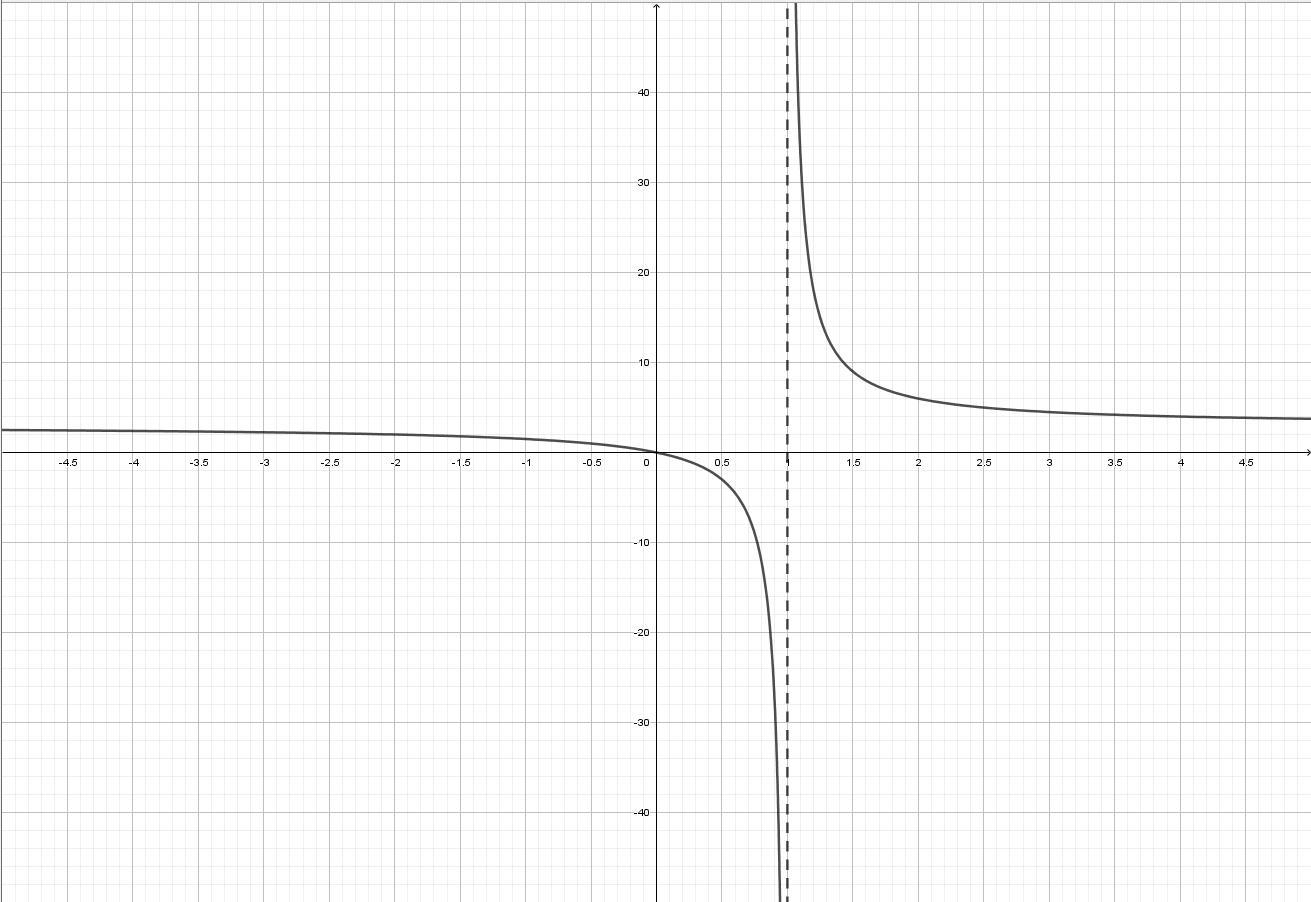
\includegraphics[width=3in]{Rat1.png}
	\end{frame}

	\begin{frame}{Domain of Rational Functions}
		Find the domain of $f(x) = \dfrac{8x + 5}{x^2 - 8x - 9}$ and discuss the behavior of $f$ near any excluded values. \pause
		
		Domain: $x \neq -1, 9 = (-\infty, -1) \cup (-1, 9) \cup (9,\infty)$ \pause
		
		\begin{tabular}{c|cccccc}
			$x$ & $ -2 $ & $-1.5$ & $-1.1$ & $-1.01$ & $-1.001$ & $\to -1$ \\ \hline
			$f(x)$ & $-1$ & $-1.33$ & $-3.76$ & $-30.76$ & $-300.76$ & $-\infty$ 
		\end{tabular} \pause
	
		\begin{tabular}{c|cccccc}
			$x$ & $0$ & $-0.5$ & $-0.9$ & $-0.99$ & $-0.999$ & $-1 \leftarrow$ \\ \hline
			$f(x)$ & $-0.56$ & $-0.21$ & $2.22$ & $29.23$ & $299.23$ & $\infty$
		\end{tabular} \pause
	
	\begin{tabular}{c|cccccc}
		$x$ & $ 8 $ & $8.5$ & $8.9$ & $8.99$ & $8.999$ & $\to 9$ \\ \hline
		$f(x)$ & $-7.67$ & $-15.36$ & $-76.96$ & $-769.9$ & $-7699$ & $-\infty$
	\end{tabular} \pause

	\begin{tabular}{c|cccccc}
		$x$ & $ 10 $ & $9.5$ & $9.1$ & $9.01$ & $9.001$ & $9 \leftarrow$ \\ \hline
		$f(x)$ & $7.73$ & $15.43$ & $77.03$ & $770.02$ & $7700$ & $\infty$
	\end{tabular}
	\end{frame}

	\begin{frame}{Domain of Rational Functions}
		Based on the tables, we draw the following conclusions:
		
		\underline{As $x$ approaches $-1$} \pause \\
		From the left: $f(x) \to -\infty$ \\
		From the right: $f(x) \to \infty$ \pause
		
		\underline{As $x$ approaches $9$} \pause \\
		From the left: $f(x) \to -\infty$ \\ \pause
		From the right: $f(x) \to \infty$ 
	\end{frame}
	
	\begin{frame}{Asymptotes}
		An \textit{asymptote} is a line that the graph of a function will approach but never cross. There are horizontal and vertical asymptotes. \pause
		
		\begin{block}{Definitions of Vertical and Horizontal Asymptotes}
			The line $x = a$ is a \textit{vertical asymptote} when $f(x) \to \infty$ or $f(x) \to -\infty$ as $x \to a$, either from the right or from the left. \vspace{12pt}
			
			The line $y = b$ is a \textit{horizontal asymptote} when $f(x) \to b$ as $x \to \infty$ or $x \to -\infty$
		\end{block} \pause
	
		In the last example, $f(x)$ had vertical asymptotes at $x = -1$ and at $x = -9$
	\end{frame}

	\begin{frame}{Asymptotes of Rational Functions}
		\begin{block}{Vertical and Horizontal Asymptotes}
			Let $f$ be the rational function \vspace{-8pt} $$f(x) = \dfrac{N(x)}{D(x)} = \dfrac{a_nx^n + a_{n-1}x^{n-1} + a_2x^2 + a_1x + a_0}{b_mx^m + b_{m-1}x^{m-1} + b_2x^2 + b_1x + b_0}$$ \vspace{-8pt} where $N(x)$ and $D(x)$ have no common factors. \vspace{8pt} \pause
			\begin{enumerate}[1)]
				\item The graph of $f$ has vertical asymptotes at the zeros of $D(x)$. \pause
				\item The graph of $f$ has at most one horizontal asymptote determined by comparing the degrees of $N(x)$ and $D(x)$. \begin{enumerate}[(a)]
					\item If $n < m$, then $f$ has the line $y = 0$ as a horizontal asymptote. \pause
					\item If $n = m$, then $f$ has the line $y = \frac{a_n}{b_m}$ as a horizontal asymptote. \pause
					\item If $n > m$, then $f$ has no horizontal asymptote.
				\end{enumerate}
			\end{enumerate}
		\end{block}
	\end{frame}

	\begin{frame}{Asymptotes of Rational Functions}
		Find all vertical and horizontal asymptotes of the graph of $f(x) = \dfrac{5x^2}{x^2 - 1}$. \pause
		
		First, factor the denominator so that we can find any vertical asymptotes:
		
		$f(x) = \dfrac{5x^2}{(x+1)(x-1)}$
		
		\pause Since the denominator is $0$ when $x = 1$ and when $x = -1$, these two lines are vertical asymptotes of the graph of $f$.
		
		\pause To find the horizontal asymptote (if there is one), we compare the degrees of each polynomial. \pause Both the numerator and denominator have a degree of $2$, so $n = m$. \pause So we know that there will be a horizontal asymptote at $y = \frac{a_n}{b_m} = \frac{5}{1} = 5$.
	\end{frame}

	\begin{frame}{Asymptotes of Rational Functions}
		Find all vertical and horizontal asymptotes of the graph of $f(x) = \dfrac{3x^2 + 7x - 6}{x^2 + 4x + 3}$. \pause
		
		First, we need to factor the numerator and denominator to see if they have any common factors: \pause
		
		$f(x) = \dfrac{(3x-2)(x+3)}{(x+1)(x+3)} = \dfrac{3x-2}{x+1}, x\neq -3$ \pause
		
		So the graph will have a vertical asymptote at $x = -1$ and a horizontal asymptote at $y = \frac{3}{1} = 3$.
	\end{frame}

	\begin{frame}{Asymptotes of Rational Functions}
		Find all asymptotes of the graph of $f(x) = \dfrac{3x}{x^2 - 4}$. \pause
		
		Factoring the denominator, we see that the graph will have vertical asymptotes at $x = 2$ and at $x = -2$. \pause
		
		Since $n < m$, the graph will have a horizontal asymptote at $y = 0$. \vspace{12pt} \pause
		
		Find all asymptotes of the graph of $g(x) = \dfrac{7x^2 - 5}{2x + 1}$. \pause
		
		There is a vertical asymptote at $x = -\frac12$. \pause
		
		Since $n > m$, there is no horizontal asymptote.
	\end{frame}

	\begin{frame}{Applications}
		The cost $C$ (in millions of dollars) of removing $p\%$ of the industrial and municipal pollutants discharged into a river is given by $C = \dfrac{255p}{100-p}, 0\leq p \leq 100$. \begin{enumerate}[a)]
			\item Find the cost of removing 80\% of the pollutants.
			\item According to the model, is it possible to remove 100\% of the pollutants? Explain.
		\end{enumerate} \pause
	
		a) $C(80) = \dfrac{255(80)}{100 - 80} = 1020$. It will cost \$1020 million, or \$1,020,000,000 to remove 80\% of the pollutants. \pause
		
		b) No, it is not possible because there is a vertical asymptote at $p = 100$.
	\end{frame}

	\begin{frame}{Applications}
		A business has a cost function of $C = 0.4x + 8000$, where $C$ is measured in dollars and $x$ is the number of units produced. The average cost per unit is given by $$\overline{C} = \dfrac{C}{x} = \dfrac{0.4x + 8000}{x}, x\geq 0$$ \begin{enumerate}[a)]
			\item Find the average cost per unit when $x = 1000$, $x = 20000$, and $x = 100000$.
			\item What is the horizontal asymptote of the graph? What does it represent?
		\end{enumerate}
	\end{frame}

	\begin{frame}{Applications}
		$\overline{C} = \dfrac{0.4x + 8000}{x}$
		
		a) Find the average cost per unit when $x = 1000$, $x = 20000$, and $x = 1000000$. \pause
		
		$\overline{C}(1000) = \dfrac{0.4(1000) + 8000}{1000} = 8.40$ \pause
		
		$\overline{C}(20000) = \dfrac{0.4(20000) + 8000}{20000} = 0.80$ \pause
		
		$\overline{C}(100000) = \dfrac{0.4(100000) + 8000}{100000} = 0.48$ \pause
		
		Interpretation: When the level of production is 1000 units, the average production cost per unit is \$8.40. When production rises to 20000 units, average cost decreases to \$0.80. At a production level of 100000 units, the average cost per item is \$0.48.
	\end{frame}

	\begin{frame}{Frame Title}
		$\overline{C} = \dfrac{0.4x + 8000}{x}$
		
		b) What is the horizontal asymptote of the graph? What does it represent? \pause
		
		The degree of the numerator and denominator are the same. The horizontal asymptote is $y = \frac{0.4}{1} = 0.4$. \pause
		
		Interpretation: No matter how many items are produced, the average cost per item will never reach \$0.40.
	\end{frame}

	\begin{frame}{Next Steps}
		\begin{itemize}
			\item Post questions in Lesson 15 Forum, if you have any
			\item Complete Assignment \#7
			\item Begin Module 9
			\begin{itemize}
				\item Read 4.2
				\item Watch Video Lesson \#16
			\end{itemize}
		\end{itemize}
	
		\vfill
		
		Thanks for watching!
	\end{frame}
\end{document}